\chapter{Estudo do Estado da Arte}
\label{chap:metod}
Nessa pesquisa foram abordados diversos aspectos que envolvem a concepção de um projeto envolvelmento um UAV do tipo quadrotor. O desenvolvimento de uma plataforma desse tipo ainda envolve desafios estruturais, autonomia, controle, localização entre outros, que necessitam de estudo prévio detalhado para ser alcançado um bom resultado com o veículo.

% %--------- NEW SECTION ----------------------
\section{Quadrotores}
% \label{sec:ui}
Quadrotores são aeronaves de asas rotativas, ou seja, são sustentandas e movimentadas por rotores. Diferente das aeronaves de asas fixas, como aviões, os aeronaves de asas rotativas não utilizam seu movimento horizontal para sustentar seu vôo. Isso faz com que esse tipo de veículo apresente um consumo energético muito maior. Apesar disso, as aeronaves de asas rotativas possuem a habilidade de realizar pouso e decolagem vertical, além de poder realizar vôos estacionários.

As aeronaves de asas rotativas são classificadas como multirotores, sendo seus tipos mais importantes quadrotores, hexarotores, octarotores, coaxiais ou helicópteros. Os quadrotores são veículos que apresentam alta manobrabilidade e alto payload, mas apresentam também alto gasto energético, tornando baixa o seu tempo de vôo, sendo um desafio achar baterias mais efieciente que aumentem sua autonomia. A medida que aumenta-se o número de rotores, passando de quadrotores para hexarotores e octarotores, aumenta-se também o payload, que é o quanto a aeronave consegue carregar em relação ao seu peso, e a tolerância a falha, que é continuar realizando um vôo controlado mesmo com algumas das hélices apresentando falhas de funcionamento. Entretanto, diminui-se também a manobrabilidade e aumenta-se o consumo energético.


Os movimentos do quadrotor são obtidos através da combinação das velocidades angulares dos rotores. Para balancear o contra-torque gerado por seus propulsores, é necessário ter a velocidade de um par de rotores que estão em uma mesma haste com o sentido horário, enquanto o outro par de rotores girando no sentido anti-horário. Para um quadrotor em realizar movimento verticais é necessário aumentar ou diminuir a velocidade dos quatro rototores simultâneamente. Para um quadrotor de translação horizontal, é necessário manter a velocidade de rotação de um par de rotores igual, enquanto a velocidade de rotação do outro par de rotores no sentido do movimento é desbalanceada, fazebdo com que o quadrotor se incline, no caso de um quadrotor em configuração em "+". Para realizar o movimento de rotação em torno do eixo vertical, conhecido como movimento de guinada. é necessário que a velocidade de um par de rotores seja superior a velocidade de rotação do outro par, fazendo com que o contra-torque resultante não seja nulo.

\subsection{Classificações}
Os quadrotores são classificados em diversas categorias, possuindo cada uma delas caracacterísticas específicas, que podem ajudar no design do projeto e também na escolha de componentes que vão ajudar na operação da aeronave.

\subsubsection{Classificação Quanto ao Peso}
L. Brooke-Holland, Unmanned Aerial Vehicles (drones): An Introduction, House of

Os UAVs são classificados em diversas categorias de acordo com o quanto eles pesam. UAVs que pesam até 2 quilogramas (kg) são classificados como micro, de 2 kg até 7 kg são classificados como mini, de 7 kg até 25 kg são classificados como pequenos, de 25 kg até 150 kg, como médios e de 150 kg em diante são classificados como grandes.\\
Quadrotores mais leves são mais ágeis por serem menores e por isso terem inércias menores. Possuindo assim maiores. acelerações angulares 

\subsubsection{Classificação Quanto a Configuração}
Os quadrotores tem duas configurações possíveis em relação à disposição de seus rotores. Os rotores podem ter a a configração em forma de "+", em que a frente da aeronave fica alinhada com uma das hastes que suporta um par de rotores. Essa configuração também é conhecida como cruz. A outra confuração possível é a configuração em "x", em que a frente da aeronave fica a 45$^{\circ}$ do eixo que contém a haste da aeronave, ficando assim a frente da aeronave no meio de duas hastes, como mostrado na Figura.

A configuração em "+" é mais acrobática, entretando, como desvantagens, a haste dos rotores bloqueia o campo de visão da câmera e também apresenta um momento de guinada ao translacionar, necessitando de um maior gasto energético para estabilizar a aeronave.

A configuração em "x" não apresenta esse efeito, por ter os movimentos de arfagem e rolagem desacoplados do de guinada. Apresenta menor esforço para transladar pois todos rotores agem nesses movimentos, diferente da configuração em "+", em que apenas um par de rotores é responsável pelo deslocamento enquanto o outro se mantém com velocidades constantes. É mais estável, entrentando apresenta menor manobrabilidade.

% \subsubsection{Ambiente de Operação}
% Os quadrotores podem operar em dois tipos de missões: outdoor e indoor. As missões outdoor são as missões em que os quadrotores são expostos a ambientes desconhecidos, onde existe a forte presença de pertubações, como rajadas de vento. Nesse tipo de missão, os quadrotores muitas vezes vão precisar de sensores do tipo GPS para ajudar na localização do veículo e também de um controlador adequado para lidar com a rejeição de pertubação. As missões indoor possuem menos pertubações e ambientes mias estruturados. Sendo possível fazer o mapeamento prévio do ambiente para realizar as operações 

\subsection{Principais Componentes}

Os principais componentes envolvidos no desenvolvilmento de um VANT do tipo quadrotor são rotores, que serão responsáveis por toda movimentação do drone, baterias, que irão garantir a energia necessária para os rotores e todos outros componentes e microcontroladores, responsáveis pela integração de hardware e de calcular as ações de controle.

\subsubsection{Sensores Inerciais}

Os VANTs são geralmente equipados com uma IMU (Inertial Measurement Unit), que são dispositivos compostos por giroscópios, acelerômetros e magnetômetros. Os giroscópios são sensores capazes de medir a velocidade angular do veículo nos três eixos, os acelerômetros são responsáveis por calcular as acelerações lineares nos três eixos e o magnetômetro mede campos magnéticos nos três eixos. Devido ao forte campo magnético existente no planeta Terra, é possível obter a orientação do robô também através da obtenção da magnitude do campo magnético atuando no eixos da aeronave. Através da fusão sensorial é possível obter a atitude do robô e realizar odometria. Muita vezes também são utilizados sensores do tipo barômetro, que são sensores capazes de medir a pressão atmosférica. Como a pressão atmosférica varia com a altitude, é possível mensurar a altura da aeronave em relação ao nível do mar da aeronave com a utilização desse sensor.

\subsubsection{Motores}

Falar sobre hélices?

Devido a alimentação do quadrotor ser a base de baterias de corrente contínua é adequado que sejam utilizados motores com esse tipo de corrente. Os motores DC são máquinas elétricas de corrente contínua (CC) que são constituídos por uma armadura ou rotor que é a parte giratória montada sobre o eixo da máquina, um estator de material ferromagnetico envolvido pelo enrolamento de campo, um comutador com função de manter o torque gerado em um determinado sentido e de escovas, que são conectores fixos que permitem o deslizamento do comutador no eixo da armadura. enrolamento de armadura. Os motores DC possuem uma grande variabilidade de velocidade de operação, podendo operar acima e abaixo do valor nominal, possuem alta aceleração, podendo varias de velocidade rapidamente, inclusive mantendo o torque constante e não necessitam de conversores complexos. Como desvantagens, eles necessitam de manutenção constante para a troca de escovas, são mais caros e maiores do que motores CA com mesma potência e também possuem centelhamento.

O motor brushless DC (BLDC) é um motor de corrente contínua síncrono que é alimentado por corrente contínua (CC) e não possui escovas de contato elétrico. Ele é composto por imãs permanentes, chamados de magnetos, que podem ser localizados no estator externo ou no centro no estator interno. A vantagem desse tipo de motor é que eles são altamente eficientes, pois possuem menos perdas por atrito, resultando em torques maiores. Essa eficiência é de grande valia para os quadrotores, pois um grande desafio associado a operação com esse tipo de veículo é a autonomia. A redução do atrito também faz com que a vida útil desse tipo de motor seja maior e que seja necessário ter menos manutenções, por não necessitar trocar as escovas.

\subsubsection{Baterias}

Um grande desafio a ser enfrentado no trabalho com veículos aéreos de asas rotativas é a autonomia. Graças ao grande gasto energético que essas aeronaves possuem para se sustentar no ar o tempo de vôo desses veículos acaba se tornando baixo.   

As baterias mais amplamente utilizadas para UAVs são baterias polímero de lítio (LiPo). Esse tipo de bateria tem uma das melhores relações entre capacidade e peso, o que é de vital importância para esse tipo de veículo, já que o peso das baterias é algo em torno de 50\% do peso da aeronave. As baterias LiPo possuem uma capacidade regular e um bom ciclo de vida. Em (Abdilla, 2015) é feito um estudo do consumo de energia de multirrotores e uma modelagem para estimação da autonomia do veículo operando com baterias LiPo.  

\subsubsection{Microcontrolador}

O microcontrolador é responsável por realizar a comunicação entre componentes e funcionalidades e a implementação do controlador que irá atuar nos propulsores. Existem diversos modelos no mercado, com diferentes frequências de operação ou clock, memória flash, RAM, EEPROM e tensão de alimentação. O clock determina quantas operações o microprocessador consegue fazer por unidade de tempo, quanto maior essa velocidade, menor é o tempo entre ações de controle, tornando o controle mais preciso. Entre as prataformas mais utilizadas estão o Arduino, a Raspberry, ARM, PIC, ESP32 e Teensy. A plataforma Arduino é baseada em chips ATmega, chegando a frequência máxima de 84 Mhz em seu modelo Arduino DUE, com SRAM de 96 kB e memória flash de 512 kB. A plataforma Raspberry Pi utiliza chips ARM, sendo seu modelo raspberry Pi 4 utilizando 4 npúcles arm com 1.5 Ghz de clock. A plataforma Teensy é baseado em chips ARM, seu modelo teensy 4.0 apresenta um chip ARM Cortex-M7 de 600mHz

\section{Revisão Bibliográfica}

Os resultados obtidos através do método BILI apresentam a rede de cocitação e os principais autores envolvidos nas pesquisas desenvolvidas no assunto abordado.

\subsection{Rede de Cocitação}

A rede de cocitação obtida mostram uma coesão. As linhas mais fortes indicam uma proximidade maior entre as pesquisas ligadas. 

\begin{figure} [h!]	
    \centering
    \caption{Método BILI}
    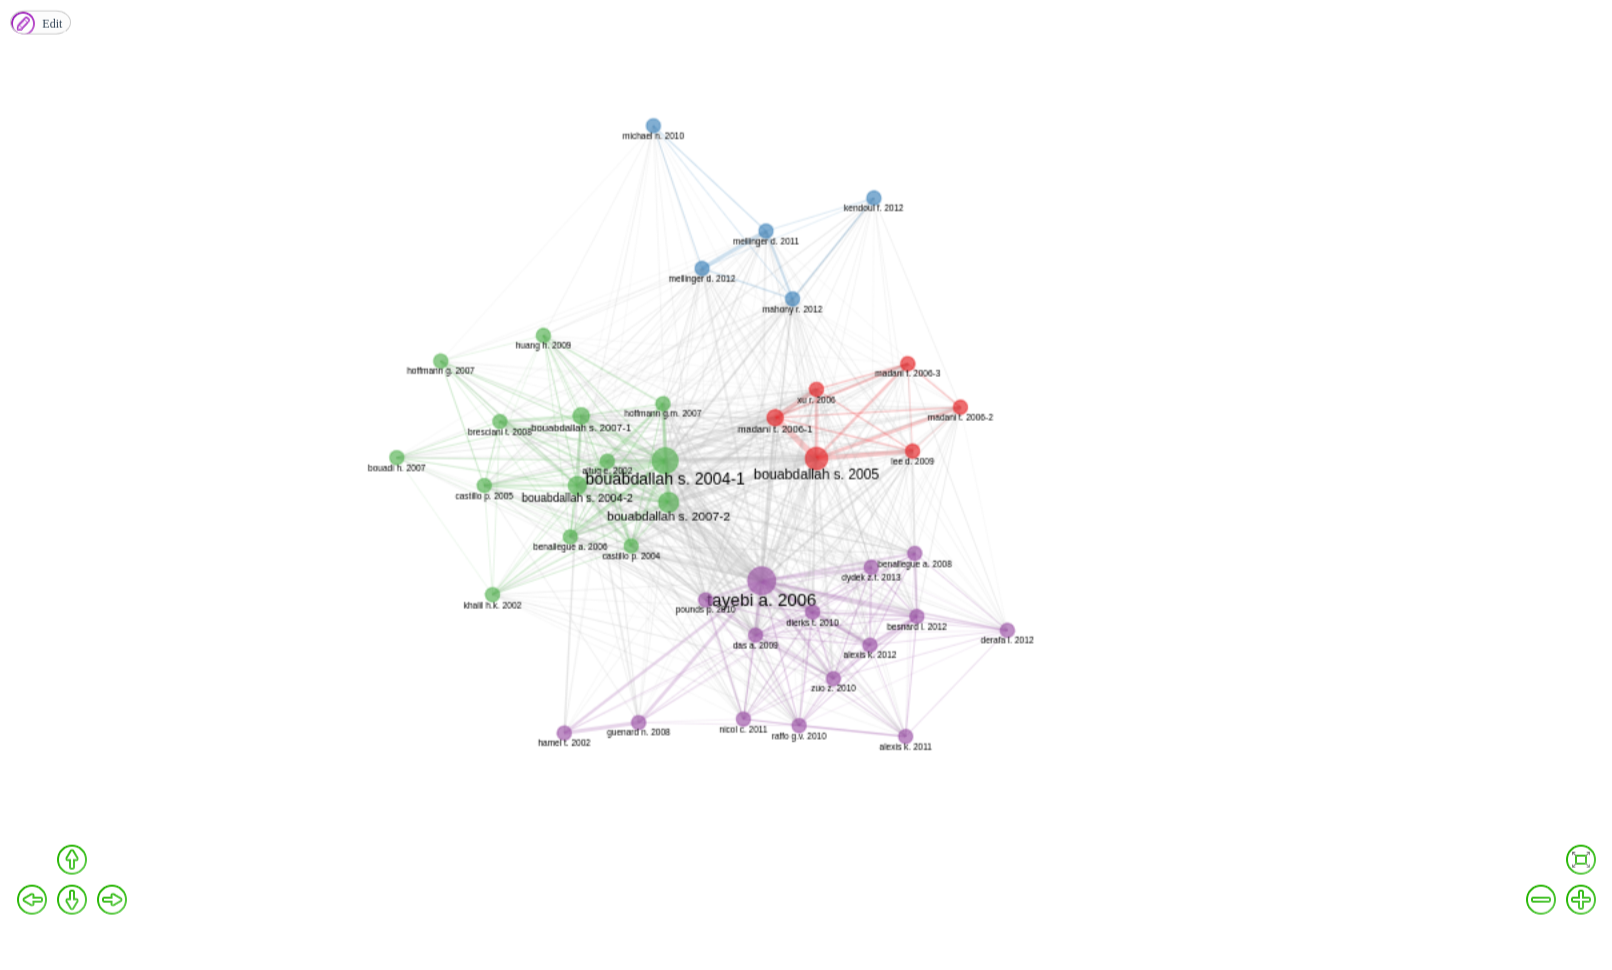
\includegraphics[width=1\textwidth]{Figures/network.png}
    \caption*{Fonte: Autoria própria.}
    \label{fig:QFD}
  \end{figure}

\subsection{Principais Autores}

Os principais autores envolvidos nas pesquisas com tema quadrotor são Kumar V., Siegwart R, Mellinger D., Bouabdallah S. e Mahony R. Bouabdalah junto com Siegwart foram um dos percursores no desenvolvimento de pesquisas sobre o design de quadrotores e controladores. Mellinger traz pesquisas na área de exploração e de planejamento de trajetória. Mahony traz pesquisas na área de pouso autônomo e Kumar diversas pesquisas com técnicas diferentes de planejamento de trajetória.

\begin{figure} [h!]	
    \centering
    \caption{Método BILI}
    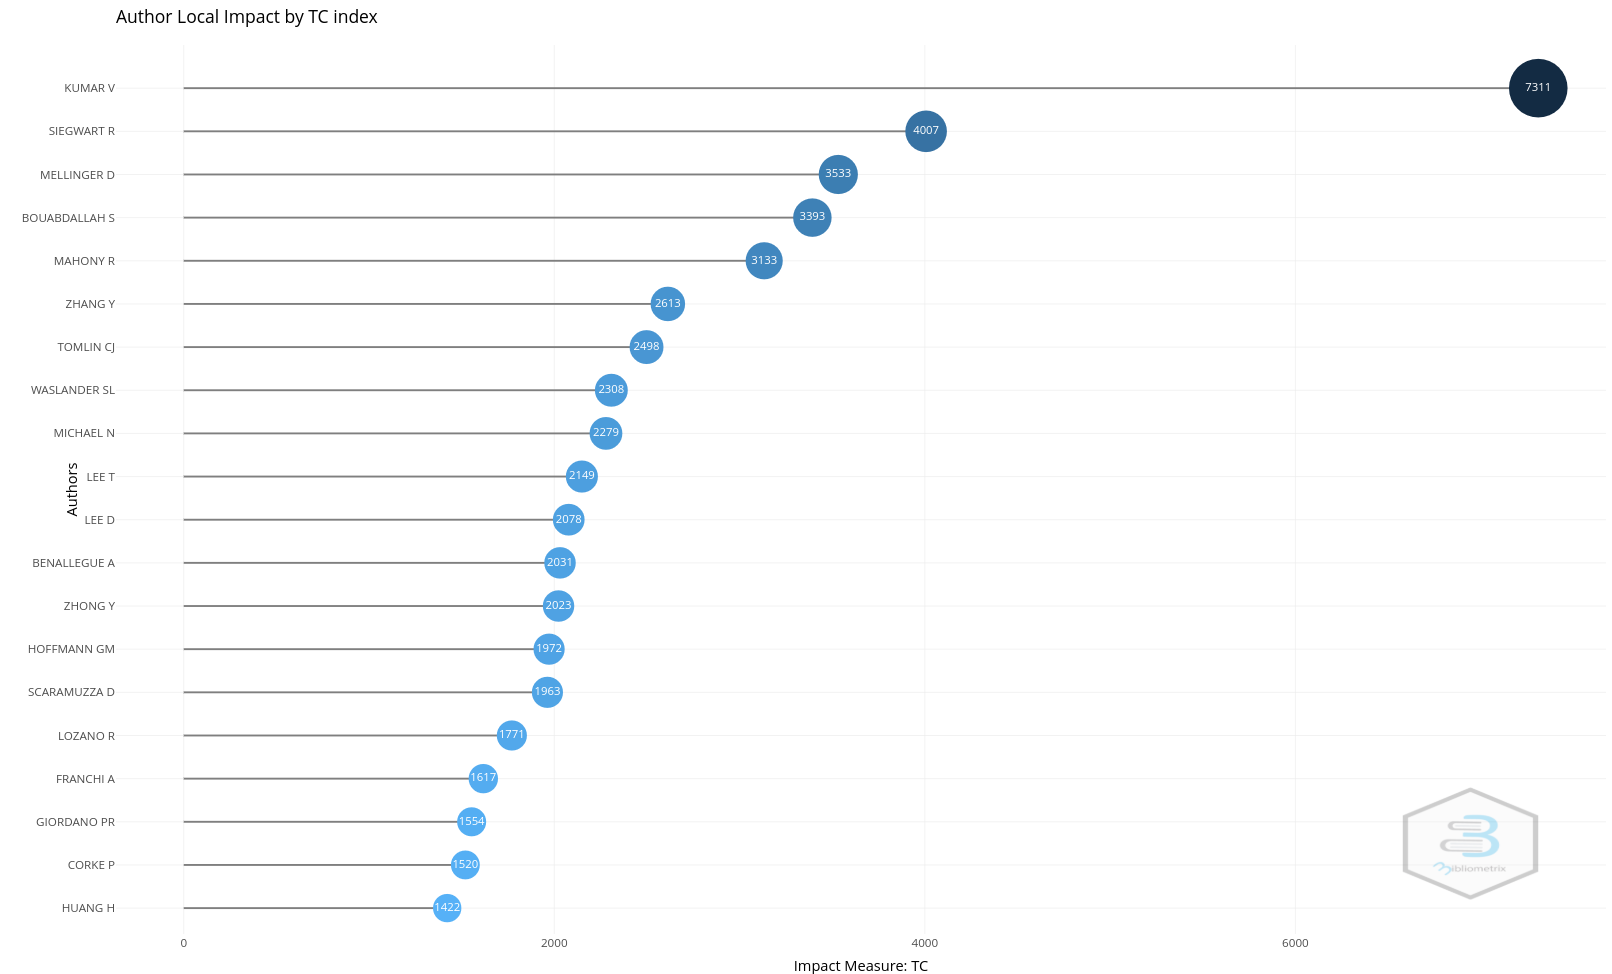
\includegraphics[width=1\textwidth]{Figures/newplot.png}
    \caption*{Fonte: Autoria própria.}
    \label{fig:QFD}
  \end{figure}

\section{Funcionalidades}
% \label{sec:ui}

\subsection{Modelagem}
A modelagem de um quadrotor é uma das etapas mais importantes no desenvolvimento de um projeto envolvendo esse tipo de veículo. Por ser uma plataforma instável, se torna inviável realizar técnicas de identificação em malha aberta. Sendo assim, é necessário obter o modelo dinâmico da aeronave através de técnicas de modelagem.

A modelagem da aeronave pode ser obtida através das equações de Newton-Euler ou através do formalismo de Euler-Lagrange (CASTILLO 2005). Através dessa modelagem é possível obter o modelo de alto nível, onde os torques e forças são entradas e as saídas são posições angulares e lineares. 

\subsection{Controle}
Os quadrotores são veículos subatuadas, ou seja, possuem mais graus de liberdade do que atuadores, são naturalmente instáveis e apresentam comportamento não-linear. Devido a esses fatores, esse tipo de veículo necessita de uma estrutura de controle adequada bem ajustada para que sejá possível a estabilização e o seguimento de referência.

Os controladores que atuam no quadrotor geralmente são utilizados em cascata (NONAMI,2010), de forma que existe um controle de baixo nível para garantir uma velocidade de rotação desejada nos rotores, um controlador em um npivel mais alto para controlar a altitude e as velocidade angulares de rolagem, arfagem e rolagem e por último um controlador no nível mais alto controladando posições lineares no espaço tridimensional. (kendoul)

Controlador hierárquico, estabilidade global

Os controlador mais comumente usado em baixo nível para controlar a velocidade de de roatação dos propulsores é o PID. 

Os controladores que controlam atitude, altitude e posições lineares no quadrotor podem ser controladores lineares ou não-lineares. Para serem utilizados controladores lineares é necessário realizar uma linearização do modelo matemático do quadrotor, considerando pequenas variações de ângulo.

Os controladores lineares que são mais amplamente utilizados são os controladores PID, LQR, H2, H$\infty$ e controle adaptativo. Como alguns parãmetros do quadrotor podem apresentar incertezas ou até mesmo variar durante a operação, também é possível adcionar robustez a esses controladores, podendo ajudar também na rejeição de pertubação. O controlador PID é um controlador prático e de fácil implementação que pode ser usado sem o conhecimento da dinâmica do sistema ajustando os parâmetros empiricamente. A técnica foi uma das primeiras a ser utilizada e é constantemente utilizada como parâmetro de comparação para outras técnicas. Foi implementado com sucesso em trabalho como (Bouabdalah 2004), (hoofman 207).

O Regulador Quadrático Linear (LQR) é um controlador de realimentação de estado que minimiza uma função custo que pondera o sinal de controle e o erro do segmento de referência. Foi incialmente implementado em Bouabdalha 2004... em waslander 2005 

O controlador H$\infty$ é um controlador por realimentação de estado que minimiza a norma H$\infty$ através da solução de desigualdades matriciais lineares. O quesito de robustez pode ser facilmente adcionado nessa técnica solucionando o problema de otimização para um politopo convexo. O controlador se mostra eficiente em lidar com pertubações. Em raffo 2008, é utilizado um controlador H$\infty$ não linear robusto para estabilizar a orientação da aeronave enquanto a técnica de Backstepping é utilizada para controlar as posições se mostrando eficiente para controlar o sistema com a presença de perturbações e incertezas paramétricas. A ação integral também pode ser uitilizada para aprimimorar os resultados, como mostrado em raffo 2010.


Os controladores não-lineares mais amplamente utilizados são os controladores por in
versão de modelo, o sliding mode control (SMC) e o controlador Fuzzy.

A técnica de sliding mode control (SMC) é um método de controle não-linear baseado do critério de estabildiade de lyapunov, que atinge seu objetivo através da definição de uma superfície de deslizamento onde estararão as trajetórias do sistema que são atingidas através de funções de chaveamento.O SMC é uma técnica que une robustez com velocidade de convergência, o que permite a aeronave realizar missões de difíceis trajetórias, lidar com grandes variações de parâmetros e pertubações. A técnica SMC também permite contruir um observador de estados, para aplicações em que a medição de determinados pode se encontrar ausente ou falhar por alguns instantes. Em (Zhao,2018) foi utilizada a um SMC adaptativo utilizando a técnica de backstepping um quadrotor e comparados os resultados com o PID e com o SMC padrão em ambiente simulacional, mostando melhores resultados o SMC adaptativo.

A técnica Backstepping é uma técnica de controle não linear recursiva baseada também no critério de Lyapunov, que obtêm um controlador que estabiliza a aeronave formalmente. Essa é uma técnica que se encaixa bem em uma arquitetura de controle em cascata cumprindo a função de controlador de atitude. A técnica se mostra eficiente para lidar com o controle da orientação da aeronave na presença de fortes pertubações.

O controlador Fuzzy é feitod e tal forma que entradas e saídas são mapeadas através da definição de funçôes de pertencimento. Em (SAntos,2010) é aplicado um controlador Fuzzy em um quadrotor para controlar a orientação da aeronave e a altitude, enquanto as entradas era a potência designada para cada motor. A técnica Fuzzy pode ser combinada com outras técnicas de controle também. Em (Nicol C.) é utilizada uma técnica chamada Cerebellar Model Articulation Controller  (CMAC) que garante um aprendizado e adaptação rápida. O CMAC associa rede neural, com técnica fuzzy e controle adaptativo. A técnica se mostrou ser computacionalmente eficiente, mas sendo necessário ajustes para adicionar robustez. Em Deepak Gautam é utilizado um PID com auto tunning dos parâmetros através de algoritmo Fuzzy. Foram obtidos resultados melhores doi que um controlador PID segundo o critério de integral do erro quadrático.


\subsection{Localização}
A localização do quadrotor pode ser auxiliada por uso de diversos sensores como LiDAR, GPS, IMU, câmeras monoculares, sensores ultrassônicos e lasers.

A IMU pode ser utilizada para a funcionalidade de localização através da odometria. A IMU pode contar com giroscópio, acelerômetro, magnetômetro e até mesmo barômetro.

Os sensores que são mais amplamente utilizados atualmente são os sensores baseados em visão. É possível obter bons resultados apenas utilizando câmeras monoculares, como mostrado em ... utilizando o pacote ORB Slam.

Os sensores GPS são amplamente utilizados para missões outdoor e os sensores ultrassônicos e baseados em laser são utilizados para auxiliar na medição da altitude.

Pode-se realizar a fusão sensorial de diversos sensores para se obter uma boa estimativa da localização da aeronave. A técnica mais amplamente utilizada é a de filtragem, como a do filtro estendido de kalman, EKF, porém ela sofre com o drift, que é um deslocamento não considerado pela medição. Outra opção é o ? framework de otimização não-linear, que apresenta resultados mais consistentes, porém apresenta um custo computacional superior.

\subsection{Planejamento de Trajetória}
O planejamento de trajetória é fundamental para que o quadrotor se torne uma plataforma completamente autônoma. Através dessa funcionalidade o veículo pode calcular uma rota para se deslocar da sua posição atual até uma posição final sem a interferência humana, sendo de extrema importância para o objetivo final do projeto que é tornal o drone capaz de realizar um pouso autônomo em uma plataforma móvel.

Diversas técnicas de planejamento de trajetória tem sido usados para lidar com o problema Belief Roadmap (onde eu vi?), A*, algoritmo? genéticos, e algoritmos com inteligência artificial

Em (v. Roberge 2013) (smiluação) foi feito um estudo de comparação entre o planejamento de trajeoria através do algoritmo genético e da otimização por enxame de partículas. explicar as técnicas.
Ambas as técnicas aprtesentaram boas soluções em tempos computacionais relativamente curtos (quanto?). Como conclusão foi observado que com significância estatística o GA apresenta melhores trajetórias ao PSO. Para comparar os resultados foi realizar o t-teste sobre o a função custo

Em (Y CHEM,2014) é feito o planejamento de trajetória através da técnica Artificial Potential Field, que é vantajosa por ser implementada através de um algoritmo de estrutura simples, com uma descrição matemática conscistente e conveniente para controle em tempo real, além de possuir uma grande portabilidade, podendo solucionar o problema de desvio de obstáculos mudando a fonte do campo potencial artificial.  (Y CHEM,2014). A técnica também pode ser utilizada para o planejamento de trajetória de vôo em formações de múltiplos UAVs. Apesar das diversas vantagens, o APF na configuração padrão não resulta na trajetória ótima, sendo possível ser combinado com outras técnicas como o algoritmo genético ou algoritmos evolucionários para melhorar seus resultados. FALAR de NMPC? O APF é baseado na idéia de que o destino funciona como um campo potencial atrativo para o UAV, enquanto os obstáculos funcionam como campos potenciais repulsivos. Nessa pesquisa, o APF é reconstruído sobre a otimização com restrições introduzida com a força de controle adicional.

Em (Y Chem,2015), é utilizada um algoritmo de de otimização derivado do Central Force Optimizatin (CFO), chamado de Modified Central Force Optimization. O CFO é um algoritmo de otimização de partícula inteligente baseado na lei da gravidade, onde cada solução é uma partícula. As partículas se atraem com a força gravitacional virtual. As massas dessas partículas são dependendes da função custo de cada solução. Na metáfora do CFO, quando uma massa está sobre forte influência de uma massa, ela fica presa em seu campo gravitacional, o que é análogo a localizar um valor máximo para uma função objetivo.
No MCFO são adcionados conceitos da otimização por Enxame de partículas (PSO) além do operador de mutação do algoritmo genético (GA) para melhorar os resultados do CFO. Os resultados da poesquisa mostraram resultados em simulação superiores aos das técnicas com o algoritmo CFO, GA, PSO e de bucas aleatórias. FA? tambem.

Em (muller 2015), é apresentado um método computacional mente eficiente que calcula trajetórias com funções de posição polinomiais três vezes diferenciáveis, considerando as retrições de velocida e aceleração do veículo. O algoritmo foi testado com a captura de uma bola arremessada pelo quadrotor.
 
% \begin{itemize}
%     \item Artificial potential field
%     \item probabilistic roadmap
%     \item belief roadmap
%     \item potential fields (PF)
%     \item Heuristic search algorithms
%     \item Optimization methods
%     \item planning under uncertainties
%     \item reactive and bio-inspired obstacle avoidance methods
% \end{itemize}



\section{Mapa Conceitual}
% \label{sec:ui}